\setcounter{ex}{0}
\setcounter{bt}{0}

% =========================================================================
% CHUYÊN ĐỀ: ỨNG DỤNG HỆ THỨC LƯỢNG TRONG TAM GIÁC VÀO CÁC BÀI TOÁN THỰC TẾ
% (DẠNG CÂU CUỐI PHẦN TỰ LUẬN - TOÁN 10 KNTT)
% =========================================================================

% --- BÀI 1 ---
\begin{ex}
	Một ngọn hải đăng có chân $H$ và đỉnh đèn $T$, được dựng vuông góc với mặt nước biển. Từ hai chiếc ca nô neo đậu tại hai vị trí $A$ và $B$ cách nhau $60\text{ m}$ trên mặt biển, người ta đo được các góc $\widehat{HAB} = 45^\circ$, $\widehat{HBA} = 60^\circ$ và góc nâng nhìn lên đỉnh đèn từ vị trí $A$ là $\widehat{HAT} = 30^\circ$. Bỏ qua chiều cao của dụng cụ đo. Hãy tính chiều cao $HT$ của ngọn hải đăng (làm tròn kết quả đến hàng phần mười của mét).
	\begin{center}
		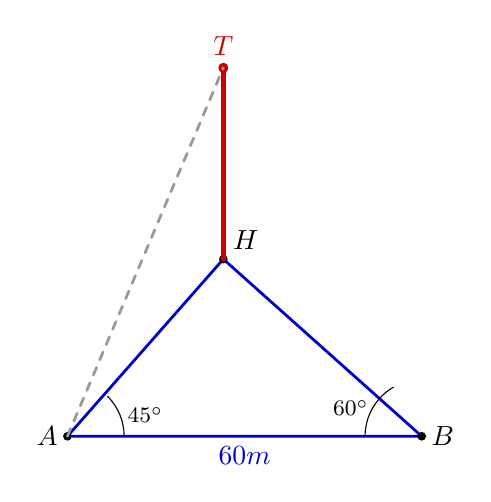
\begin{tikzpicture}[scale=0.9, line join=round, line cap=round]
			% Mặt nước biển
			\coordinate (A) at (0,0);
			\coordinate (B) at (5,0);
			\coordinate (H) at (2.2, 2.5);
			\coordinate (T) at (2.2, 5.2);
			
			% Tam giác ABH trên mặt biển
			\draw[line width=1pt, blue!80!black] (A) -- (B) node[midway, below] {$60\text{ m}$} -- (H) -- cycle;
			\filldraw[black] (A) circle (1.5pt) node[left] {$A$};
			\filldraw[black] (B) circle (1.5pt) node[right] {$B$};
			\filldraw[black] (H) circle (1.5pt) node[above right] {$H$};
			
			% Ngọn hải đăng HT
			\draw[line width=2pt, red!80!black] (H) -- (T) node[above] {$T$};
			\filldraw[red!80!black] (T) circle (1.8pt);
			
			% Đường ngắm AT
			\draw[line width=1pt, dashed, gray!80] (A) -- (T);
			
			% Kí hiệu góc
			\draw (0.8,0) arc (0:45:0.8);
			\node at (1.1,0.3) {\footnotesize $45^\circ$};
			\draw (4.2,0) arc (180:120:0.8);
			\node at (4.0,0.4) {\footnotesize $60^\circ$};
		\end{tikzpicture}
	\end{center}
	\loigiai{
		Trong tam giác $ABH$ nằm trên mặt biển, ta có:
		$$\widehat{AHB} = 180^\circ - (\widehat{HAB} + \widehat{HBA}) = 180^\circ - (45^\circ + 60^\circ) = 75^\circ.$$
		Áp dụng định lí sin trong tam giác $ABH$, ta có:
		$$\dfrac{AH}{\sin\widehat{HBA}} = \dfrac{AB}{\sin\widehat{AHB}} \implies AH = \dfrac{AB \cdot \sin 60^\circ}{\sin 75^\circ} = \dfrac{60 \cdot \dfrac{\sqrt{3}}{2}}{\sin 75^\circ} \approx 53{,}79\text{ (m)}.$$
		Xét tam giác vuông $AHT$ vuông tại $H$ (do ngọn hải đăng dựng thẳng đứng vuông góc với mặt nước):
		$$HT = AH \cdot \tan\widehat{HAT} = AH \cdot \tan 30^\circ \approx 53{,}79 \cdot \dfrac{1}{\sqrt{3}} \approx 31{,}1\text{ (m)}.$$
		Vậy chiều cao của ngọn hải đăng xấp xỉ $31{,}1\text{ m}$.
	}
\end{ex}

% --- BÀI 2 ---
\begin{ex}
	Hai trạm kiểm soát ven biển $A$ và $B$ cách nhau $15\text{ km}$. Tại thời điểm ban đầu, trạm quan sát phát hiện một tàu đánh cá ở vị trí $C$ thỏa mãn $\widehat{CAB} = 45^\circ$ và $\widehat{CBA} = 60^\circ$. Sau đó, con tàu di chuyển thẳng từ $C$ về phía trạm $A$ một quãng đường $4\text{ km}$ rồi dừng lại ở vị trí $D$ ($D$ nằm giữa $C$ và $A$). Hãy tính khoảng cách từ vị trí $D$ của tàu đến trạm $B$ (làm tròn kết quả đến hàng phần trăm của kilômét).
	\begin{center}
		\begin{tikzpicture}[scale=0.85, line join=round, line cap=round]
			\coordinate (A) at (0,0);
			\coordinate (B) at (7,0);
			\coordinate (C) at (4.8, 4.8);
			\coordinate (D) at ($(C)!0.3!(A)$);
			
			\draw[line width=1pt] (A) -- (B) node[midway, below] {$15\text{ km}$} -- (C) -- cycle;
			\draw[line width=1pt, blue, dashed] (B) -- (D);
			
			\filldraw[black] (A) circle (1.5pt) node[below left] {$A$};
			\filldraw[black] (B) circle (1.5pt) node[below right] {$B$};
			\filldraw[black] (C) circle (1.5pt) node[above] {$C$};
			\filldraw[red!80!black] (D) circle (1.8pt) node[above left] {$D$};
			
			\node[left, font=\footnotesize] at ($(C)!0.5!(D)$) {$4\text{ km}$};
			
			\draw (0.9,0) arc (0:45:0.9);
			\node at (1.2,0.3) {\footnotesize $45^\circ$};
			\draw (6.2,0) arc (180:120:0.8);
			\node at (6.0,0.4) {\footnotesize $60^\circ$};
		\end{tikzpicture}
	\end{center}
	\loigiai{
		Trong tam giác $ABC$, số đo góc $\widehat{ACB}$ là:
		$$\widehat{ACB} = 180^\circ - (45^\circ + 60^\circ) = 75^\circ.$$
		Áp dụng định lí sin trong tam giác $ABC$:
		$$\dfrac{AC}{\sin\widehat{CBA}} = \dfrac{AB}{\sin\widehat{ACB}} \implies AC = \dfrac{15 \cdot \sin 60^\circ}{\sin 75^\circ} \approx \dfrac{15 \cdot 0{,}8660}{0{,}9659} \approx 13{,}45\text{ (km)}.$$
		Vì điểm $D$ thuộc đoạn $AC$ và $CD = 4\text{ km}$ nên:
		$$AD = AC - CD = 13{,}45 - 4 = 9{,}45\text{ (km)}.$$
		Áp dụng định lí côsin trong tam giác $ABD$, ta có:
		$$BD^2 = AB^2 + AD^2 - 2AB \cdot AD \cdot \cos\widehat{BAD} = 15^2 + (9{,}45)^2 - 2 \cdot 15 \cdot 9{,}45 \cdot \cos 45^\circ$$
		$$\implies BD^2 \approx 225 + 89{,}30 - 283{,}5 \cdot 0{,}7071 \approx 113{,}84 \implies BD \approx 10{,}67\text{ (km)}.$$
		Vậy khoảng cách từ vị trí $D$ đến trạm $B$ khoảng $10{,}67\text{ km}$.
	}
\end{ex}

% --- BÀI 3 ---
\begin{ex}
	Một khu bảo tồn sinh thái hình tam giác $ABC$ có $AB = 80\text{ m}$, $AC = 100\text{ m}$ và góc $\widehat{BAC} = 120^\circ$. Người ta đặt một trạm bơm nước tại đỉnh $A$ và lắp một đường ống dẫn nước thẳng từ trạm $A$ đến điểm $M$ trên cạnh $BC$ sao cho $MB = 3MC$. Hãy tính chiều dài của đường ống dẫn nước $AM$ (làm tròn kết quả đến hàng phần mười của mét).
	\begin{center}
		\begin{tikzpicture}[scale=0.9, line join=round, line cap=round]
			\coordinate (A) at (0,0);
			\coordinate (B) at (3.5,0);
			\coordinate (C) at (-2.5, 4.33); % 5*cos(120), 5*sin(120)
			\coordinate (M) at ($(B)!0.75!(C)$); % MB = 3MC => BM = 3/4 BC
			
			\draw[line width=1.1pt] (A) -- (B) node[midway, below] {$80\text{ m}$} -- (C) -- cycle;
			\node[left] at ($(A)!0.5!(C)$) {$100\text{ m}$};
			\draw[line width=1.2pt, red!80!black] (A) -- (M) node[midway, left] {$AM$};
			
			\filldraw[black] (A) circle (1.5pt) node[below left] {$A$};
			\filldraw[black] (B) circle (1.5pt) node[below right] {$B$};
			\filldraw[black] (C) circle (1.5pt) node[above left] {$C$};
			\filldraw[blue] (M) circle (1.5pt) node[above right] {$M$};
			
			\draw (0.6,0) arc (0:120:0.6);
			\node at (0.3,0.7) {\footnotesize $120^\circ$};
		\end{tikzpicture}
	\end{center}
	\loigiai{
		Áp dụng định lí côsin trong tam giác $ABC$, độ dài cạnh $BC$ là:
		$$BC^2 = AB^2 + AC^2 - 2AB \cdot AC \cdot \cos 120^\circ = 80^2 + 100^2 - 2 \cdot 80 \cdot 100 \cdot \left(-\dfrac{1}{2}\right) = 24\,400$$
		$$\implies BC = \sqrt{24\,400} \approx 156{,}20\text{ (m)}.$$
		Áp dụng hệ quả của định lí côsin để tính góc $\widehat{B}$:
		$$\cos B = \dfrac{AB^2 + BC^2 - AC^2}{2AB \cdot BC} = \dfrac{80^2 + 24\,400 - 100^2}{2 \cdot 80 \cdot \sqrt{24\,400}} = \dfrac{20\,800}{160 \cdot 156{,}20} \approx 0{,}8323.$$
		Do điểm $M$ nằm trên cạnh $BC$ và $MB = 3MC$ nên $MB = \dfrac{3}{4}BC \approx 117{,}15\text{ m}$.\\
		Áp dụng định lí côsin trong tam giác $ABM$:
		$$AM^2 = AB^2 + MB^2 - 2AB \cdot MB \cdot \cos B \approx 80^2 + (117{,}15)^2 - 2 \cdot 80 \cdot 117{,}15 \cdot 0{,}8323 \approx 4\,524{,}1$$
		$$\implies AM = \sqrt{4\,524{,}1} \approx 67{,}3\text{ (m)}.$$
		Vậy chiều dài của đường ống dẫn nước $AM$ xấp xỉ $67{,}3\text{ m}$.
	}
\end{ex}

% --- BÀI 4 ---
\begin{ex}
	Một khu đất hình tam giác $ABC$ có $AB = 120\text{ m}$, $BC = 160\text{ m}$ và góc $\widehat{ABC} = 115^\circ$. Người ta muốn làm một lối thoát hiểm thẳng ngắn nhất từ vị trí $B$ đến tuyến đường chạy dọc cạnh $AC$. Hãy tính chiều dài của lối thoát hiểm này (làm tròn kết quả đến hàng phần mười của mét).
	\begin{center}
		\begin{tikzpicture}[scale=0.85, line join=round, line cap=round]
			\coordinate (B) at (0,0);
			\coordinate (A) at (4,0);
			\coordinate (C) at (-2.25, 4.8);
			\coordinate (H) at ($(A)!(B)!(C)$); % Hinh chieu cua B len AC
			
			\draw[line width=1.1pt] (A) node[below right] {$A$} -- (B) node[below left] {$B$} -- (C) node[above] {$C$} -- cycle;
			\draw[line width=1.2pt, red!80!black] (B) -- (H) node[above right] {$H$};
			\draw (H) rectangle ++(-0.25,-0.2);
			
			\node[below] at ($(A)!0.5!(B)$) {$120\text{ m}$};
			\node[left] at ($(B)!0.5!(C)$) {$160\text{ m}$};
			
			\draw (0.6,0) arc (0:115:0.6);
			\node at (0.3,0.5) {\footnotesize $115^\circ$};
		\end{tikzpicture}
	\end{center}
	\loigiai{
		Khoảng cách ngắn nhất từ $B$ đến cạnh $AC$ chính là độ dài đường cao $BH$ hạ từ $B$ xuống đường thẳng $AC$.\\
		Vì $\widehat{ABC} = 115^\circ > 90^\circ$ nên hai góc $\widehat{A}$ và $\widehat{C}$ đều là góc nhọn, do đó chân đường cao $H$ luôn nằm trong đoạn thẳng $AC$.\\
		Áp dụng định lí côsin trong tam giác $ABC$:
		$$AC^2 = AB^2 + BC^2 - 2AB \cdot BC \cdot \cos 115^\circ = 120^2 + 160^2 - 2 \cdot 120 \cdot 160 \cdot \cos 115^\circ$$
		$$\implies AC^2 \approx 14\,400 + 25\,600 - 38\,400 \cdot (-0{,}4226) = 56\,228 \implies AC \approx 237{,}12\text{ (m)}.$$
		Diện tích của tam giác $ABC$ là:
		$$S = \dfrac{1}{2}AB \cdot BC \cdot \sin\widehat{ABC} = \dfrac{1}{2} \cdot 120 \cdot 160 \cdot \sin 115^\circ \approx 8\,700{,}5\text{ (m}^2\text{)}.$$
		Mặt khác, $S = \dfrac{1}{2}AC \cdot BH \implies BH = \dfrac{2S}{AC} \approx \dfrac{2 \cdot 8\,700{,}5}{237{,}12} \approx 73{,}4\text{ (m)}$.\\
		Vậy chiều dài của lối thoát hiểm xấp xỉ $73{,}4\text{ m}$.
	}
\end{ex}

% --- BÀI 5 ---
\begin{ex}
	Hai vị trí quan sát $A$ và $B$ trên bờ sông cách nhau $100\text{ m}$. Một trạm phát sóng $C$ ở phía bên kia bờ sông thỏa mãn các góc $\widehat{CAB} = 50^\circ$ và $\widehat{CBA} = 70^\circ$. Một kỹ sư di chuyển từ vị trí $A$ đến điểm $D$ trên đoạn $AB$ sao cho $AD = 40\text{ m}$ và hướng ống ngắm dọc theo tia $DB$. Hỏi kỹ sư phải quay ống ngắm về phía trạm $C$ một góc bằng bao nhiêu độ? (Tính số đo góc $\widehat{CDB}$, làm tròn kết quả đến hàng phần mười của độ).
	\begin{center}
		\begin{tikzpicture}[scale=0.9, line join=round, line cap=round]
			\coordinate (A) at (0,0);
			\coordinate (B) at (6,0);
			\coordinate (C) at (4.2, 5.0);
			\coordinate (D) at (2.4, 0);
			
			% Bờ sông
			\draw[line width=1pt] (-0.5,0) -- (6.8,0) node[right, font=\footnotesize] {Bờ sông};
			\draw[line width=1.1pt, blue] (A) -- (C) -- (B);
			\draw[line width=1.2pt, red!80!black] (D) -- (C);
			
			\filldraw[black] (A) circle (1.5pt) node[below] {$A$};
			\filldraw[black] (B) circle (1.5pt) node[below] {$B$};
			\filldraw[black] (C) circle (1.5pt) node[above] {$C$};
			\filldraw[black] (D) circle (1.5pt) node[below] {$D$};
			
			\node[below] at ($(A)!0.5!(D)$) {\footnotesize $40\text{ m}$};
			\draw[<->, dashed] ([yshift=-12pt]A) -- ([yshift=-12pt]B) node[midway, fill=white, font=\footnotesize] {$100\text{ m}$};
			
			\draw (0.8,0) arc (0:50:0.8);
			\node at (1.1,0.3) {\footnotesize $50^\circ$};
			\draw (5.2,0) arc (180:110:0.8);
			\node at (5.0,0.4) {\footnotesize $70^\circ$};
			
			\draw (2.9,0) arc (0:70:0.5);
			\node at (3.1,0.35) {\footnotesize $?$};
		\end{tikzpicture}
	\end{center}
	\loigiai{
		Trong tam giác $ABC$, ta có số đo góc $\widehat{ACB}$ là:
		$$\widehat{ACB} = 180^\circ - (50^\circ + 70^\circ) = 60^\circ.$$
		Áp dụng định lí sin trong tam giác $ABC$:
		$$\dfrac{AC}{\sin 70^\circ} = \dfrac{AB}{\sin 60^\circ} \implies AC = \dfrac{100 \cdot \sin 70^\circ}{\sin 60^\circ} \approx \dfrac{100 \cdot 0{,}9397}{0{,}8660} \approx 108{,}51\text{ (m)}.$$
		Xét tam giác $ADC$ có $AD = 40\text{ m}$, $AC = 108{,}51\text{ m}$ và $\widehat{CAD} = 50^\circ$.\\
		Áp dụng định lí côsin trong tam giác $ADC$:
		$$CD^2 = AD^2 + AC^2 - 2AD \cdot AC \cdot \cos 50^\circ \approx 40^2 + (108{,}51)^2 - 2 \cdot 40 \cdot 108{,}51 \cdot \cos 50^\circ \approx 7\,794{,}5$$
		$$\implies CD \approx 88{,}29\text{ (m)}.$$
		Áp dụng định lí sin trong tam giác $ADC$ để tìm góc $\widehat{ADC}$:
		$$\dfrac{CD}{\sin 50^\circ} = \dfrac{AC}{\sin\widehat{ADC}} \implies \sin\widehat{ADC} = \dfrac{AC \cdot \sin 50^\circ}{CD} \approx \dfrac{108{,}51 \cdot 0{,}7660}{88{,}29} \approx 0{,}9414.$$
		Vì trong tam giác $ADC$ ta có $AC > CD$ ($108{,}51 > 88{,}29$) nên góc đối diện $\widehat{ADC}$ là góc tù, suy ra:
		$$\widehat{ADC} \approx 180^\circ - 70{,}3^\circ = 109{,}7^\circ.$$
		Do đó, góc quay cần tìm là:
		$$\widehat{CDB} = 180^\circ - \widehat{ADC} = 180^\circ - 109{,}7^\circ = 70{,}3^\circ.$$
	}
\end{ex}

% --- BÀI 6 ---
\begin{ex}
	Để đo khoảng cách giữa hai vị trí $C$ và $D$ ở bờ bên kia của một con sông, một nhóm đo đạc thiết lập hai điểm mốc $A$ và $B$ ở bờ bên này sao cho $AB = 80\text{ m}$. Bằng thiết bị ngắm, người ta đo được các góc: $\widehat{CAB} = 85^\circ$, $\widehat{DAB} = 35^\circ$, $\widehat{CBA} = 40^\circ$ và $\widehat{DBA} = 75^\circ$. Hãy tính khoảng cách giữa hai vị trí $C$ và $D$ (làm tròn kết quả đến hàng phần mười của mét).
	\begin{center}
		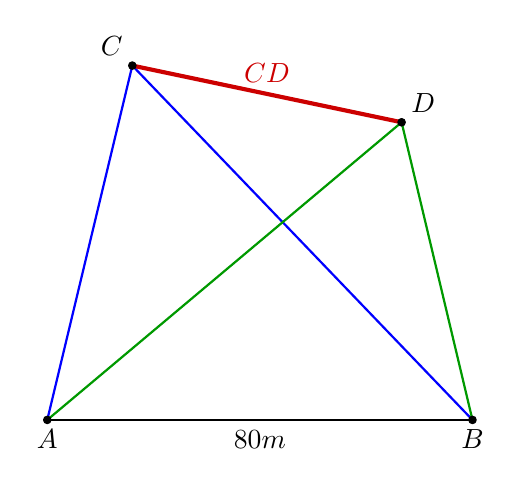
\begin{tikzpicture}[scale=0.9, line join=round, line cap=round]
			\coordinate (A) at (0,0);
			\coordinate (B) at (6,0);
			\coordinate (C) at (1.2, 5.0);
			\coordinate (D) at (5.0, 4.2);
			
			% Các đường nối
			\draw[line width=1pt] (A) -- (B) node[midway, below] {$80\text{ m}$};
			\draw[line width=0.8pt, blue] (A) -- (C) -- (B);
			\draw[line width=0.8pt, green!60!black] (A) -- (D) -- (B);
			\draw[line width=1.5pt, red!80!black] (C) -- (D) node[midway, above] {$CD$};
			
			\filldraw[black] (A) circle (1.5pt) node[below] {$A$};
			\filldraw[black] (B) circle (1.5pt) node[below] {$B$};
			\filldraw[black] (C) circle (1.5pt) node[above left] {$C$};
			\filldraw[black] (D) circle (1.5pt) node[above right] {$D$};
		\end{tikzpicture}
	\end{center}
	\loigiai{
		\begin{itemize}
			\item Trong tam giác $ABC$: $\widehat{ACB} = 180^\circ - (\widehat{CAB} + \widehat{CBA}) = 180^\circ - (85^\circ + 40^\circ) = 55^\circ$.\\
			Áp dụng định lí sin trong tam giác $ABC$:
			$$\dfrac{AC}{\sin 40^\circ} = \dfrac{AB}{\sin 55^\circ} \implies AC = \dfrac{80 \cdot \sin 40^\circ}{\sin 55^\circ} \approx \dfrac{80 \cdot 0{,}6428}{0{,}8192} \approx 62{,}77\text{ (m)}.$$
			\item Trong tam giác $ABD$: $\widehat{ADB} = 180^\circ - (\widehat{DAB} + \widehat{DBA}) = 180^\circ - (35^\circ + 75^\circ) = 70^\circ$.\\
			Áp dụng định lí sin trong tam giác $ABD$:
			$$\dfrac{AD}{\sin 75^\circ} = \dfrac{AB}{\sin 70^\circ} \implies AD = \dfrac{80 \cdot \sin 75^\circ}{\sin 70^\circ} \approx \dfrac{80 \cdot 0{,}9659}{0{,}9397} \approx 82{,}23\text{ (m)}.$$
			\item Trong tam giác $ACD$, ta có $\widehat{CAD} = \widehat{CAB} - \widehat{DAB} = 85^\circ - 35^\circ = 50^\circ$.\\
			Áp dụng định lí côsin trong tam giác $ACD$:
			$$CD^2 = AC^2 + AD^2 - 2AC \cdot AD \cdot \cos 50^\circ$$
			$$CD^2 \approx (62{,}77)^2 + (82{,}23)^2 - 2 \cdot 62{,}77 \cdot 82{,}23 \cdot \cos 50^\circ \approx 4\,068{,}2 \implies CD \approx 63{,}8\text{ (m)}.$$
		\end{itemize}
		Vậy khoảng cách giữa hai điểm $C$ và $D$ xấp xỉ $63{,}8\text{ m}$.
	}
\end{ex}

% --- BÀI 7 ---
\begin{ex}
	Để xác định chiều cao của một ngọn núi so với mặt đất nằm ngang, người ta chọn hai điểm quan sát $A$ và $B$ thẳng hàng với chân núi $H$, cùng nằm về một phía so với núi và cách nhau $500\text{ m}$. Từ $A$ và $B$, người ta đo được góc nâng nhìn lên đỉnh núi $S$ lần lượt là $\widehat{SAH} = 34^\circ$ và $\widehat{SBH} = 42^\circ$ (điểm $B$ ở gần chân núi hơn). Bỏ qua chiều cao của dụng cụ đo. Hãy tính chiều cao $SH$ của ngọn núi (làm tròn kết quả đến hàng đơn vị của mét).
	\begin{center}
		\begin{tikzpicture}[scale=0.9, line join=round, line cap=round]
			\coordinate (A) at (0,0);
			\coordinate (B) at (3.5,0);
			\coordinate (H) at (6.5,0);
			\coordinate (S) at (6.5,3.2);
			
			% Đất và núi
			\draw[line width=1pt] (-0.5,0) -- (7.5,0) node[right, font=\footnotesize] {Mặt đất};
			\draw[line width=1.5pt, brown!70!black] (H) -- (S) node[above] {$S$ (Đỉnh núi)};
			\draw (H) rectangle ++(-0.25,0.25);
			
			% Tia ngắm
			\draw[line width=1pt, blue] (A) -- (S);
			\draw[line width=1pt, blue] (B) -- (S);
			
			\filldraw[black] (A) circle (1.5pt) node[below] {$A$};
			\filldraw[black] (B) circle (1.5pt) node[below] {$B$};
			\filldraw[black] (H) circle (1.5pt) node[below] {$H$};
			
			\draw[<->, dashed] ([yshift=-10pt]A) -- ([yshift=-10pt]B) node[midway, fill=white, font=\footnotesize] {$500\text{ m}$};
			
			\draw (0.8,0) arc (0:34:0.8);
			\node at (1.1,0.3) {\footnotesize $34^\circ$};
			\draw (4.2,0) arc (0:42:0.7);
			\node at (4.5,0.35) {\footnotesize $42^\circ$};
		\end{tikzpicture}
	\end{center}
	\loigiai{
		Trong tam giác $SAB$, góc $\widehat{SBH}$ là góc ngoài tại đỉnh $B$ nên:
		$$\widehat{ASB} = \widehat{SBH} - \widehat{SAH} = 42^\circ - 34^\circ = 8^\circ.$$
		Áp dụng định lí sin trong tam giác $SAB$:
		$$\dfrac{SB}{\sin\widehat{SAB}} = \dfrac{AB}{\sin\widehat{ASB}} \implies SB = \dfrac{500 \cdot \sin 34^\circ}{\sin 8^\circ} \approx \dfrac{500 \cdot 0{,}5592}{0{,}1392} \approx 2\,008{,}6\text{ (m)}.$$
		Xét tam giác vuông $SBH$ vuông tại $H$:
		$$SH = SB \cdot \sin\widehat{SBH} = SB \cdot \sin 42^\circ \approx 2\,008{,}6 \cdot 0{,}6691 \approx 1\,344\text{ (m)}.$$
		Vậy chiều cao của ngọn núi so với mặt đất xấp xỉ $1\,344\text{ m}$.
	}
\end{ex}

% --- BÀI 8 ---
\begin{ex}
	Cùng một lúc từ một cảng biển $O$, hai tàu thủy bắt đầu xuất phát chạy theo hai hướng khác nhau tạo với nhau một góc $60^\circ$. Tàu thứ nhất chạy với vận tốc trung bình $24\text{ km/h}$, tàu thứ hai chạy với vận tốc trung bình $30\text{ km/h}$. Giả sử hai tàu giữ nguyên hướng và tốc độ không đổi. Hỏi sau $2$ giờ di chuyển, khoảng cách giữa hai con tàu bằng bao nhiêu kilômét? (Làm tròn kết quả đến hàng phần mười của kilômét).
	\begin{center}
		\begin{tikzpicture}[scale=0.9, line join=round, line cap=round]
			\coordinate (O) at (0,0);
			\coordinate (A) at (4,0);
			\coordinate (B) at (2.5, 4.33); % 5*cos(60), 5*sin(60)
			
			\draw[->, line width=1.2pt, blue] (O) -- (A) node[midway, below] {$48\text{ km}$} node[right] {Tàu 1 ($A$)};
			\draw[->, line width=1.2pt, green!60!black] (O) -- (B) node[midway, left] {$60\text{ km}$} node[above right] {Tàu 2 ($B$)};
			\draw[line width=1.2pt, red!80!black, dashed] (A) -- (B) node[midway, above right] {$?$};
			
			\filldraw[black] (O) circle (1.5pt) node[below left] {$O$ (Cảng)};
			\draw (0.8,0) arc (0:60:0.8);
			\node at (0.6,0.4) {\footnotesize $60^\circ$};
		\end{tikzpicture}
	\end{center}
	\loigiai{
		Sau $2$ giờ di chuyển, quãng đường mỗi tàu đi được lần lượt là:
		\begin{itemize}
			\item Quãng đường tàu thứ nhất: $OA = 24 \cdot 2 = 48\text{ (km)}$.
			\item Quãng đường tàu thứ hai: $OB = 30 \cdot 2 = 60\text{ (km)}$.
		\end{itemize}
		Áp dụng định lí côsin trong tam giác $OAB$:
		$$AB^2 = OA^2 + OB^2 - 2OA \cdot OB \cdot \cos\widehat{AOB} = 48^2 + 60^2 - 2 \cdot 48 \cdot 60 \cdot \cos 60^\circ$$
		$$AB^2 = 2\,304 + 3\,600 - 2 \cdot 48 \cdot 60 \cdot \dfrac{1}{2} = 5\,904 - 2\,880 = 3\,024$$
		$$\implies AB = \sqrt{3\,024} \approx 55{,}0\text{ (km)}.$$
		Vậy sau $2$ giờ di chuyển, khoảng cách giữa hai con tàu xấp xỉ $55{,}0\text{ km}$.
	}
\end{ex}

% --- BÀI 9 ---
\begin{ex}
	Một máy bay trực thăng cứu hộ đang bay lượn ở một độ cao cố định trên biển. Từ hai tàu cứu nạn $A$ và $B$ cách nhau $300\text{ m}$ trên mặt biển, cùng một thời điểm người ta phát hiện máy bay ở vị trí $C$ với góc nâng nhìn lên máy bay từ tàu $A$ là $\widehat{CAB} = 55^\circ$ và từ tàu $B$ là $\widehat{CBA} = 65^\circ$ (giả sử máy bay và hai tàu cùng nằm trong một mặt phẳng thẳng đứng). Hãy tính khoảng cách từ tàu cứu nạn $A$ đến trực thăng cứu hộ $C$ (làm tròn kết quả đến hàng phần mười của mét).
	\begin{center}
		\begin{tikzpicture}[scale=0.9, line join=round, line cap=round]
			\coordinate (A) at (0,0);
			\coordinate (B) at (6,0);
			\coordinate (C) at (3.5, 4.5);
			
			% Mặt biển
			\draw[line width=1pt, cyan!70!blue] (-1,0) -- (7.5,0) node[right, font=\footnotesize] {Mặt biển};
			\draw[line width=1.1pt, blue] (A) -- (C);
			\draw[line width=1.1pt, blue] (B) -- (C);
			
			\filldraw[black] (A) circle (1.5pt) node[below] {$A$ (Tàu 1)};
			\filldraw[black] (B) circle (1.5pt) node[below] {$B$ (Tàu 2)};
			\filldraw[red] (C) circle (2pt) node[above] {$C$ (Trực thăng)};
			
			\draw[<->, dashed] ([yshift=-12pt]A) -- ([yshift=-12pt]B) node[midway, fill=white, font=\footnotesize] {$300\text{ m}$};
			
			\draw (0.8,0) arc (0:55:0.8);
			\node at (1.1,0.4) {\footnotesize $55^\circ$};
			\draw (5.2,0) arc (180:115:0.8);
			\node at (5.0,0.4) {\footnotesize $65^\circ$};
		\end{tikzpicture}
	\end{center}
	\loigiai{
		Trong tam giác $ABC$, số đo góc $\widehat{ACB}$ là:
		$$\widehat{ACB} = 180^\circ - (\widehat{CAB} + \widehat{CBA}) = 180^\circ - (55^\circ + 65^\circ) = 60^\circ.$$
		Áp dụng định lí sin trong tam giác $ABC$:
		$$\dfrac{AC}{\sin\widehat{CBA}} = \dfrac{AB}{\sin\widehat{ACB}} \implies AC = \dfrac{AB \cdot \sin 65^\circ}{\sin 60^\circ} = \dfrac{300 \cdot \sin 65^\circ}{\sin 60^\circ} \approx \dfrac{300 \cdot 0{,}9063}{0{,}8660} \approx 313{,}9\text{ (m)}.$$
		Vậy khoảng cách từ tàu cứu nạn $A$ đến trực thăng cứu hộ $C$ xấp xỉ $313{,}9\text{ m}$.
	}
\end{ex}

% --- BÀI 10 ---
\begin{ex}
	Để đo khoảng cách giữa hai vị trí $A$ và $B$ ở hai đầu một hồ nước mà không thể kéo dây đo trực tiếp, người ta chọn một vị trí $C$ trên bờ có thể nhìn thấy cả hai điểm $A$ và $B$. Từ vị trí $C$, người ta đo được khoảng cách $CA = 150\text{ m}$, $CB = 200\text{ m}$ và góc $\widehat{ACB} = 75^\circ$. Hãy tính khoảng cách giữa hai vị trí $A$ và $B$ (làm tròn kết quả đến hàng phần mười của mét).
	\begin{center}
		\begin{tikzpicture}[scale=0.9, line join=round, line cap=round]
			\coordinate (C) at (0,0);
			\coordinate (A) at (4.5,0);
			\coordinate (B) at (1.55, 5.8); % 6*cos(75), 6*sin(75)
			
			% Đồ họa hồ nước mờ
			\draw[line width=1.1pt, cyan!60!blue, fill=cyan!8, smooth cycle] 
				plot coordinates {(2,1.5) (4,0.5) (4.5,2.5) (3,4.5) (1.2,3)};
			\node[cyan!70!blue, font=\bfseries\footnotesize] at (2.8,2.5) {Hồ nước};
			
			% Các đoạn thẳng
			\draw[line width=1pt] (C) -- (A) node[midway, below] {$150\text{ m}$};
			\draw[line width=1pt] (C) -- (B) node[midway, left] {$200\text{ m}$};
			\draw[line width=1.3pt, red!80!black, dashed] (A) -- (B) node[midway, above right] {$AB = ?$};
			
			\filldraw[black] (C) circle (1.5pt) node[below left] {$C$};
			\filldraw[black] (A) circle (1.5pt) node[below right] {$A$};
			\filldraw[black] (B) circle (1.5pt) node[above] {$B$};
			
			\draw (0.8,0) arc (0:75:0.8);
			\node at (0.6,0.5) {\footnotesize $75^\circ$};
		\end{tikzpicture}
	\end{center}
	\loigiai{
		Áp dụng định lí côsin trong tam giác $ABC$, ta có:
		$$AB^2 = CA^2 + CB^2 - 2CA \cdot CB \cdot \cos\widehat{ACB} = 150^2 + 200^2 - 2 \cdot 150 \cdot 200 \cdot \cos 75^\circ$$
		$$AB^2 = 22\,500 + 40\,000 - 60\,000 \cdot \cos 75^\circ \approx 62\,500 - 60\,000 \cdot 0{,}2588 = 46\,972$$
		$$\implies AB = \sqrt{46\,972} \approx 216{,}7\text{ (m)}.$$
		Vậy khoảng cách giữa hai vị trí $A$ và $B$ ở hai đầu hồ nước xấp xỉ $216{,}7\text{ m}$.
	}
\end{ex}
